\chapter{Planteamiento del Problema}
\section{Descripción de la Realidad Problemática}

A nivel mundial, las tasas de presencia de cáncer de tiroides en personas varían de acuerdo con la edad, al género y al país. En el caso de Perú se tiene que por cada 100 000 mujeres existen 10.9 de casos de incidencia en este tipo de cáncer, y por cada 100 000 varones, se tiene un 3.6 de casos. Además de los casos de incidencia, la mortalidad también está presente y varía en varias partes del mundo. En Perú la mortalidad de pacientes mujeres con cáncer de tiroides es 1.7 por cada 100 000 personas, mientras que en los varones es de 0.77 casos cada 100 000 personas. \parencite{ws_oms2022cancert}

A continuación, se presentan dos gráficos que muestran los distintos índices de incidencia y mortalidad de cáncer de tiroides en mujeres, donde se puede resaltar la presencia de Perú en los rangos más altos de cada uno de estos. 

\begin{figure}[H]
	\begin{center}
		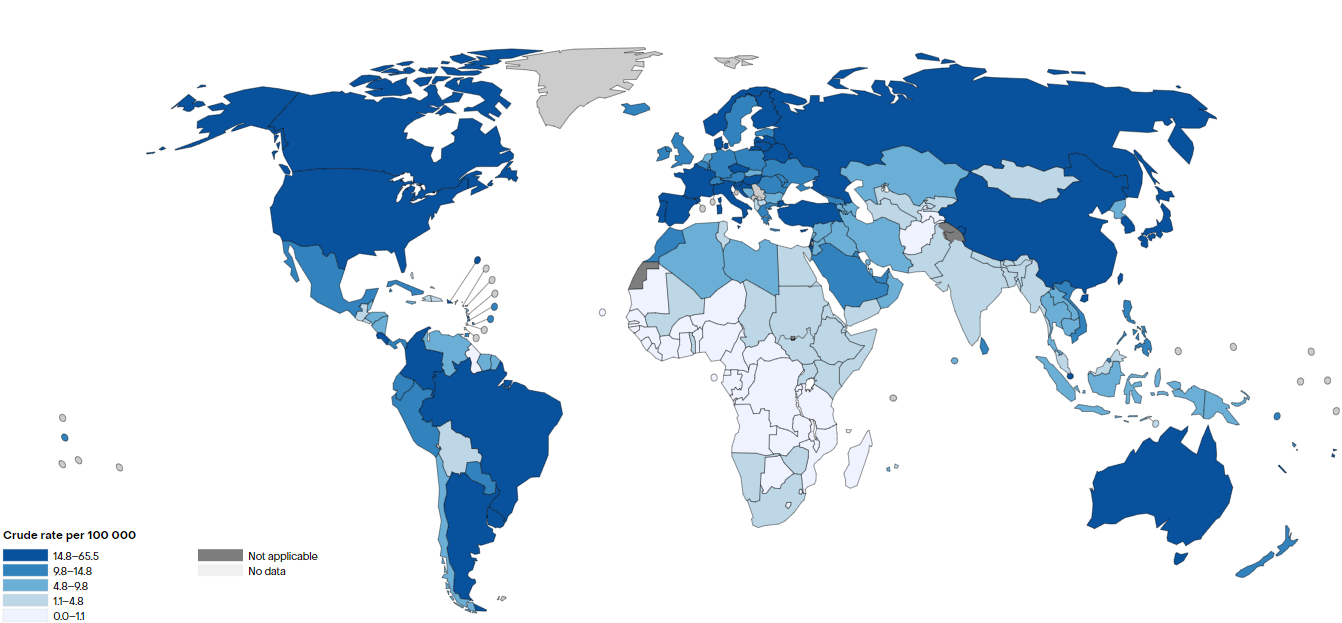
\includegraphics[width=1.00 \textwidth]{1/figures/tb_inc_ct_mujeres.png}
		\caption[Tasa bruta de incidencia de cáncer de tiroides en mujeres por 100 000 personas]{Tasa bruta de incidencia de cáncer de tiroides en mujeres por 100 000 personas. \\
		Fuente: \cite{ws_oms2022cancert}. \textit{Cancer Today}.}
		\label{1:fig}
	\end{center}
\end{figure}


\begin{figure}[H]
	\begin{center}
		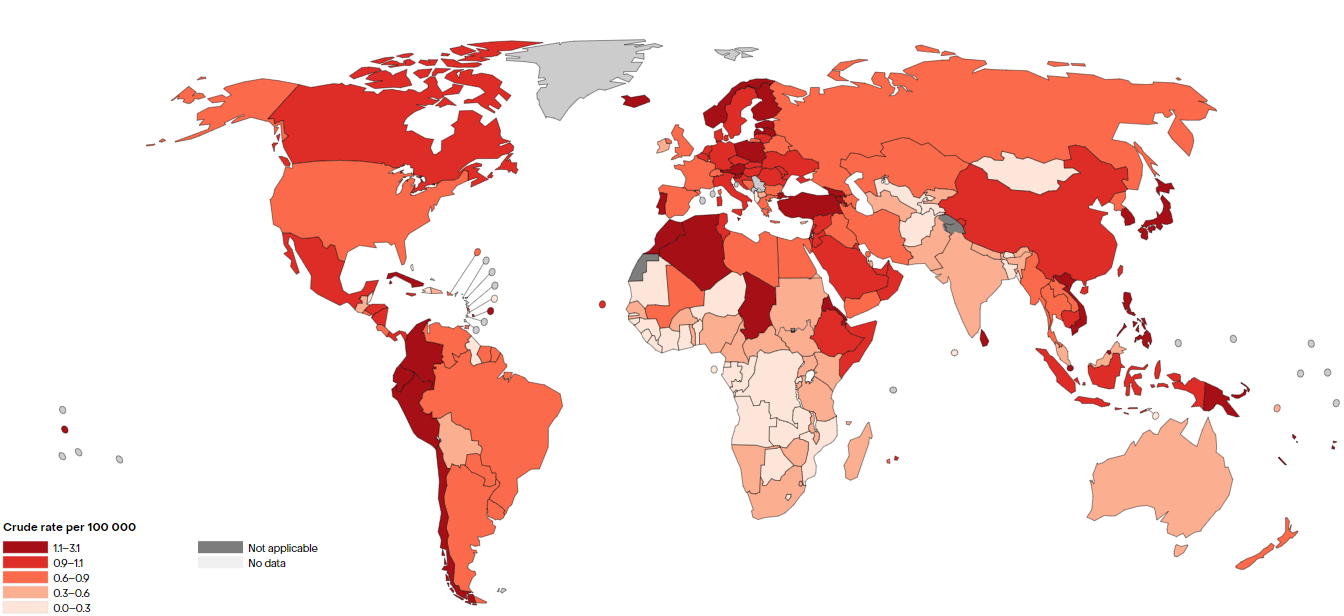
\includegraphics[width=1.00 \textwidth]{1/figures/tb_mor_ct_mujeres.png}
		\caption[Tasa bruta de mortalidad de cáncer de tiroides en mujeres por 100 000 personas]{Tasa bruta de mortalidad de cáncer de tiroides en mujeres por 100 000 personas. \\
		Fuente: \cite{ws_oms2022cancert}. \textit{Cancer Today}.}
		\label{1:fig2}
	\end{center}
\end{figure}

De igual forma, en el caso de los varones, el Perú también se encuentra entre los rangos más altos de incidencia y mortalidad. A continuación, se muestran sus respectivas gráficas.

\begin{figure}[H]
	\begin{center}
		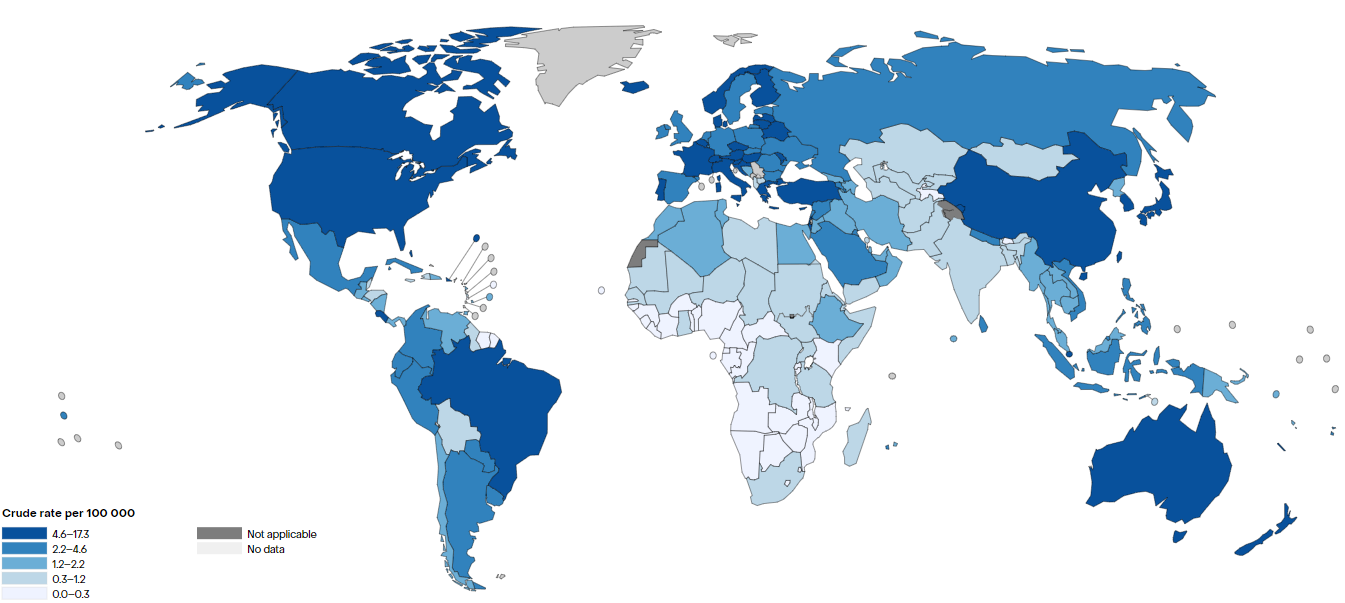
\includegraphics[width=1.00 \textwidth]{1/figures/tb_inc_ct_varones.png}
		\caption[Tasa bruta de incidencia de cáncer de tiroides en varones por 100 000 personas]{Tasa bruta de incidencia de cáncer de tiroides en varones por 100 000 personas. \\
		Fuente: \cite{ws_oms2022cancert}. \textit{Cancer Today}.}
		\label{1:fig3}
	\end{center}
\end{figure}

\begin{figure}[H]
	\begin{center}
		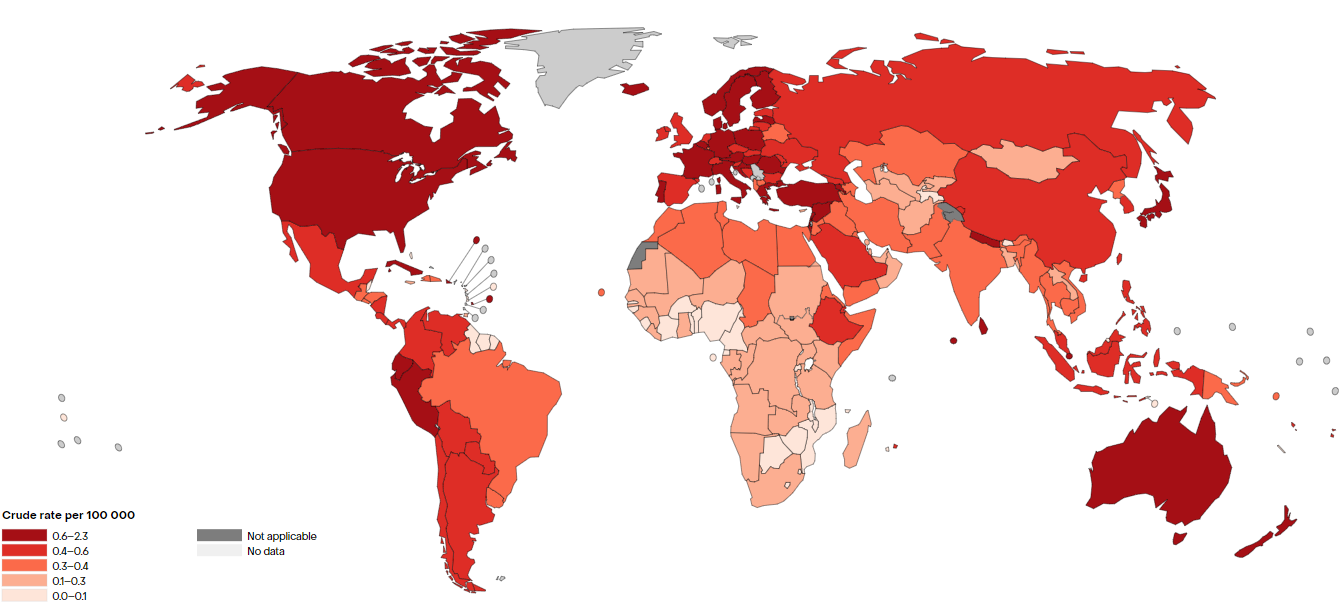
\includegraphics[width=1.00 \textwidth]{1/figures/tb_mor_ct_varones.png}
		\caption[Tasa bruta de mortalidad de cáncer de tiroides en varones por 100 000 personas]{Tasa bruta de mortalidad de cáncer de tiroides en varones por 100 000 personas. \\
		Fuente: \cite{ws_oms2022cancert}. \textit{Cancer Today}.}
		\label{1:fig4}
	\end{center}
\end{figure}

Con el siguiente gráfico que muestra los mismos índices distribuidos por género y regiones del mundo, es fácil notar la alta incidencia de este tipo de cáncer en las mujeres, siendo la región con mayor incidencia América del Norte, mientras que la de mayor mortalidad es Oceanía. La región de Latino América y el Caribe supera a Norte América en mortalidad, aunque se encuentra por debajo de Oceanía y Europa.

\begin{figure}[H]
	\begin{center}
		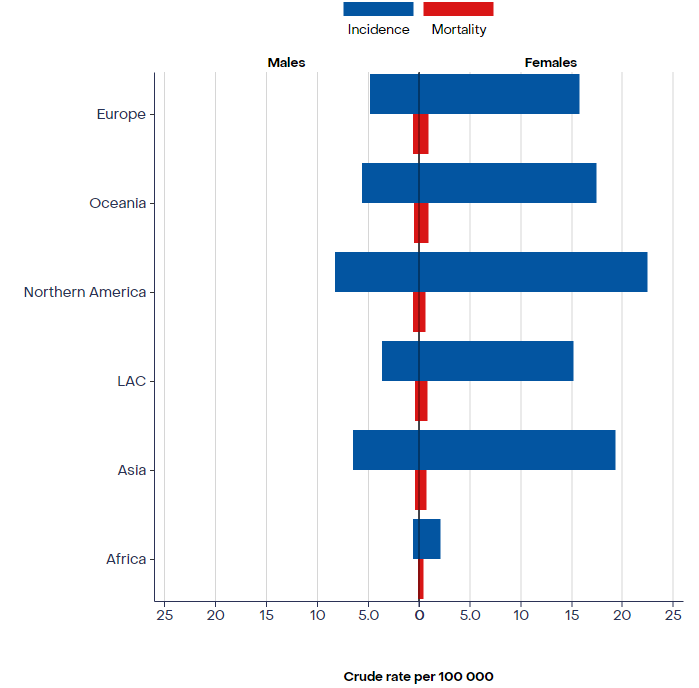
\includegraphics[width=0.60 \textwidth]{1/figures/tb_inc_mor_gen_y_reg.png}
		\caption[Tasa bruta de incidencia y mortalidad de cáncer de tiroides por género y región]{Tasa bruta de incidencia y mortalidad de cáncer de tiroides por género y región. \\
		Fuente: \cite{ws_oms2022cancert}. \textit{Cancer Today}.}
		\label{1:fig5}
	\end{center}
\end{figure}

Además, es importante mencionar que este aumento de incidencia a nivel global de cáncer de tiroides se debe a diversos factores relacionados a problemas de salud como la obesidad y a factores medioambientales como por ejemplo exposición al yodo \parencite{pr_kim2020geoinflu}. Sin embargo, otro factor es la poca disposición y capacidad de realizar un diagnóstico a tiempo de los nódulos tiroideos que, de forma general, cerca del 7\% al 15\% de los casos de llegan a ser cancerígenos \parencite{pr_haugen2016amethy}.

Para la detección temprana de este tipo de cáncer o desarrollo de tumores, depende en gran medida de la experiencia y la capacidad cognitiva de un experto en radiología, y muchos de estos se ven en la necesidad de utilizar no muy avanzados sistemas de diagnóstico por computadora, mejor conocido como CAD por sus siglas en inglés \parencite{pr_zhu2021agendlframew}. Ante grandes limitaciones de sistemas CAD básicos, y aprovechando el extenso uso de la inteligencia artificial, el Deep Learning y sus algoritmos son capaces de incorporar mayor eficacia a dichos sistemas.

El Deep Learning ha sido usado ampliamente como herramienta para el procesamiento de imágenes médicas, no solo para detectar diferentes tipos de cáncer o nódulos como los relacionados a los pulmones, sino también para la retinopatía diabética y localización de feto en ecografías, e inclusive en la detección del COVID-19 \parencite{pr_bhatta2021medimage}. Además, el aumento de la calidad de imágenes de ultrasonido que se fue desarrollando en los últimos 30 años, aumentando cada vez más resolución de las imágenes y el tiempo de adquisición, ha permitido una mejora en términos de detección de enfermedad; sin embargo, aún se requiere de un médico especializado y debidamente entrenado para lograr un realizar un correcto análisis de las imágenes, por ello se vio en la necesidad de encontrar métodos de clasificación automatizada, pero dichos métodos antiguos consumían bastante tiempo, gran poder computacional y poca capacidad de generalización de resultados, es así que en este contexto, apareció una novedosa arquitectura de Deep Learning que actualmente es usado en diferentes área el día de hoy: las Redes Neuronales Convolucionales o CNN, quitando en gran medida los problemas de las antigua técnicas \parencite{pr_signgh20203ddl}. Aunque existe varios antecedentes con esta técnica de Deep Learning en detección de nódulos en la tiroides, muy pocos se han centrado en el grado de ayuda que se brinda a un médico especialista, ya que una simple detección no aceleraría debidamente el proceso de descarte de una anomalía en la tiroides.


\section{Formulación del Problema}
Con el objetivo de formular los objetivos de esta investigación, se propusieron las siguientes preguntas.
\subsection{Problema General}
PG: \newcommand{\ProblemaGeneral}{
¿Es posible implementar un modelo de Deep Learning para el diagnóstico de nódulos tiroideos a través de imágenes de ultrasonido?
}
\ProblemaGeneral
\subsection{Problemas Específicos}
\newcommand{\Pbone}{
¿Qué características del conjunto de datos a usar para entrenar y evaluar los modelos son ideales para obtener buenos resultados?
}
\newcommand{\Pbtwo}{
¿Qué técnicas de preprocesamiento se deberían aplicar a las imágenes de ultrasonido del conjunto de datos?
}
\newcommand{\Pbthree}{
¿De qué forma se puede evaluar el rendimiento de los modelos de Deep Learning en la clasificación de imágenes de ultrasonido?
}


\begin{itemize}
	\item PE1: {\Pbone}
	\item PE2: {\Pbtwo}
	\item PE3: {\Pbthree}
\end{itemize}

\section{Objetivos de la Investigación}
A continuación, se presentan el objetivo general y los objetivos específicos.
\subsection{Objetivo General}
OG: \newcommand{\ObjetivoGeneral}{
Diseñar un modelo de Deep Learning para el de diagnóstico de nódulos tiroideos a través de imágenes de ultrasonido.
}
\ObjetivoGeneral
\subsection{Objetivos Específicos}
\newcommand{\Objone}{
Determinar las características ideales del conjunto de datos a usar para entrenar y evaluar los modelos.
}
\newcommand{\Objtwo}{
Determinar las técnicas de preprocesamiento que se deben aplicar a las imágenes de ultrasonido del conjunto de datos.
}
\newcommand{\Objthree}{
Identificar las métricas de evaluación de rendimiento de los modelos de Deep Learning en la clasificación de imágenes de ultrasonido.
}


\begin{itemize}
	\item OE1: {\Objone}
	\item OE2: {\Objtwo}
	\item OE3: {\Objthree}
\end{itemize}



\section{Justificación de la Investigación}

\subsection{Teórica}
La investigación se desarrolla con el propósito de otorgar mayor conocimiento sobre el uso de la inteligencia artificial en el diagnóstico de nódulos en la glándula de la tiroides, esto a través de imágenes de ultrasonido. Esta investigación aportará conocimiento sobre el diseño y eficacia de los sistemas de diagnóstico asistido por computadora con base en el Deep Learning en el diagnóstico de nódulos tiroideos. Esto servirá para que en un futuro se generen nuevos y más eficaces sistemas de apoyo médicos dentro de esta área.

\subsection{Práctica}
Los antecedentes presentados en la investigación califican la capacidad de un modelo de Deep Learning en la detección y diagnóstico de una imagen de ultrasonido de la tiroides, esto usando diferentes algoritmos y técnicas con el objetivo de aumentar la capacidad el modelo. Muchos de estos abarcan la parte de clasificar una imagen, mientras que otros realizan segmentación del área donde el nódulo se está desarrollando, basándose además en estándares médicos de diagnóstico. Muy pocos realizan ambos: clasificación y segmentación. La presente investigación se centrará en desarrollar un modelo de clasificación. 

\subsection{Metodológica}
El modelo desarrollado en la investigación no propone un reemplazo de los médicos especialistas en el área, sino una herramienta potente para estos que ayudará a diagnosticar los nódulos que se desarrollan en la glándula de tiroides. La investigación presentará y concluirá con las herramientas tecnológicas y técnicas de Deep Learning ideales para el desarrollo de sistemas de diagnóstico asistido por computadora, esto luego de una extensa recopilación de datos y métodos que permitan la construcción y desarrollo de un modelo eficiente y eficaz.

\section{Delimitación del Estudio}
A continuación, se presentará la delimitación espacial, temporal y conceptual.

\subsection{Espacial}
Debido a que la problemática y necesidad de diagnosticar a tiempo los nódulos tiroideos no es propio de una región o país, la mayoría de la data para realizar un correcto análisis de inteligencia artificial son basados en países extranjeros y de gran alcance como Estados Unidos, India y China. Los proyectos previos más afines al tema presentados en la investigación son desarrollados en diversos países extranjeros. 

\subsection{Temporal}
Los datos presentados en esta investigación sobre casos de incidencia y mortalidad de la tiroides son hasta el 2022. De igual forma, las imágenes de ultrasonido de glándulas de tiroides con presencia de nódulos que se usarán para entrenar y validar el modelo de clasificación son recopiladas del conjunto de datos de acceso libre TNCD recolectada hasta finales del año 2022. Los antecedentes relacionados a esta investigación fueron publicados entre el 2019 y 2023.

\subsection{Conceptual}
La presente investigación se centrará en el desarrollo de un modelo de Deep Learning para realizar la clasificación de nódulos de la glándula de tiroides y así lograr determinar si es de carácter benigno o maligno. 
